\documentclass[a4paper,11pt]{article}
\usepackage[a4paper,left=3.1cm,right=3.1cm,top=3cm,bottom=2.9cm]{geometry}
\usepackage[english]{babel}
\usepackage[utf8]{inputenc}
\usepackage{amsmath,amsthm,amssymb,amsfonts,stmaryrd, wasysym}
\usepackage{color}
\usepackage{graphicx}
\usepackage{todonotes}
\usepackage{subcaption}
\usepackage{wrapfig}
\usepackage{multirow} %multirow in table

\usepackage{algorithm}
\usepackage{algpseudocode}
\usepackage{xcolor}
\usepackage{titling}
\usepackage{caption}
\usepackage{hyperref}
\captionsetup{font=footnotesize}

\newcommand{\subtitle}[1]{%
  \posttitle{%
    \par\end{center}
    \begin{center}\large#1\end{center}
    \vskip0.5em}%
}

%%%%%%%%%%%%%%%%% Kopf- & Fußzeile %%%%%%%%%%%%%%%%%
\usepackage[footsepline]{scrlayer-scrpage}
\pagestyle{scrheadings}
\clearscrheadfoot
\title{Machine Learning - Exercise 3}
\subtitle{Model Stealing/Extraction}
\author{Christian Hatschka, Daniel Fangl, Esra Ceylan}
\date{February 2021}
\ihead{\thetitle}
\ifoot{\newline \theauthor}
\ofoot{\newline \pagemark}
\setlength{\headheight}{15pt}
\setlength{\footheight}{29pt}

%%%%%%%% Biblatex
\usepackage[backend=biber,style=numeric,sortlocale=de_DE,natbib=true,url=false, doi=true,eprint=false]{biblatex}
\addbibresource{literature.bib}

\begin{document}
\maketitle

\section{Group members}
    Daniel Fangl (01526097) has a bachelor in Software Engineering and is currently in the master course Software Engineering and Internet Computing. Christian Hatschka (01525634) and Esra Ceylan (01526801) both have a bachelor in Mathematics and are currently enrolled in the master course Logic and Computation.
    
\section{Introduction}
    As the construction of a good model is an expensive and time consuming task, the thought of training a model based on an existing but not explicitly given one is interesting. We will do this using the original model as a black-box and taking its predictions into account.
    
    The aim of this project is to extract several models by using different model-stealing methods. Moreover, we will test their efficiency and accuracy and compare their performance to the performance of the underlying original model.
    
\section{Copycat Networks for CNN}\label{sec:copycat}
    This model stealing attack was proposed by Correia-Silva et al.~\cite{copycat} and aims to copy a Convolutional Neural Network. First, we will use the target CNN as a black-box to label our training set, which can also contain instances from the non-problem domain if the model allows us to classify them. For example the Microsoft Azure Emotion API does not allow to upload instances, where it cannot detect a face, hence which are not part of the problem-domain. Even images containing a face can sometimes be rejected as the Azure API could not always detect a face. By classifying the data using the target network as black-box we create a fake data set which will be used to train the extracted model.
    
    Next, we will select a model architecture of the copycat network. A possible problem with this approach is that we might not know the model architecture of the original network. However, this should not be a big problem as the knowledge can be copied to a different model.
    As pre-trained models tend to perform better, we will use the VGG-16 architecture with pre-trained weights. It is obviously optimal if the pre-trained model is already close to the problem domain.
    
    In the next step we will use the generated fake data set to fit the pre-trained model.
    As described in~\cite{copycat} we will use Stochastic Gradient Descent with a Step Down policy for the learning rate for training the copycat model. 
    
    We carried out our experiments using an Intel Core i7 6700k with 16GB RAM and NVIDIA GeForce GTX 1070. The environment of the experiments was Arch Linux with NVIDIA CUDA 10.2 and cuDNN 7.6.5.
    
    \subsection{Data Set: Emotion Detection}
        Unfortunately, we could not get access to the data sets used in~\cite{copycat} to compare our results with the results in the paper. Therefore, we used other data sets for our experiments. We combined two sets, which are described in the following two subsections to obtain a larger number of instances.
        %As our first data set we combined the data sets described in the following two subsections. 
        %Since KDEF and AKDEF were one of the used data sets in the paper of Correia-Silva et al. we wanted to take them as validation that we achieve similar results. Unfortunately, they contain only about 5\,000 samples in total and we could not get access to other data sets used in the paper. Therefore, we combined them with a larger data set.
        
        \subsubsection{KDEF and AKDEF} \label{subsec:dataset_KDEF-AKDEF}
            The Karolinska directed emotional faces data set~\cite{kdef} (short KDEF) contains 4\,900 images of human facial expressions. The pictures were taken of 70 different people (35 male and 35 female) displaying 7 different emotional expressions. All people portrayed were amateur actors between the ages of 20 and 30 and had no facial hair, glasses or makeup during the photos. Each of the expressions were taken from multiple different angles. 
            
            The averaged Karolinska directed emotional faces data set~\cite{kdef} (short AKDEF) contains $70$ averaged images of KDEF. The averaging was done over images containing the same gender, angle and emotional expression.
            
            Both data sets contain labels and were made by the Karolinska Institute in Stockholm, Sweden by the Department of Clinical Neuroscience in 1998. The data sets have been used in a large number of research publications on the topic. 
            
        \subsubsection{Emotion Detection from Facial Expressions} \label{subsec:dataset_kaggle-emotions}
            This data set was taken from the Kaggle competition 'Emotion Detection From Facial Expressions'~\cite{kaggle-emotion}. 
            It contains 13\,690 images of several human faces with different emotions. The data set was constructed from a variety of different sources, e.g.
            \begin{itemize}
                \item labeled Faces In The Wild,
                \item the Japanese Female Facial Expression (JAFFE) Database,
                \item Indian Movie Face database (IMFDB),
                \item the Extended Yale Face Database B.
            \end{itemize}
            
            Additionally, this data set contains, like the previous one, labeled data allowing us to compare the performance of the extracted model and also the overall performance of the target network.
    
    \subsection{Microsoft Azure Emotion API}
        As our first target model we used the publicly available Microsoft Azure Emotion API. For an input image this API returns a percentage vector of emotions for each face in the image. The following emotions are measured: 
        %This API classifies the emotion a face portrays, in the form of a percentage vectors that assigns values to the following emotions:
            \begin{itemize}
                \item Anger
                \item Contempt
                \item Disgust
                \item Fear
                \item Happiness
                \item Neutral
                \item Sadness
                \item Surprise
            \end{itemize}
        For example the face in Figure~\ref{fig:happy_face} from the publicly available KDEF data set returns a vector assigning a percentage of $0.999$ to happiness, $0.001$ to surprise and $0$ to everything else.
            \begin{figure}[h!]
                    \centering      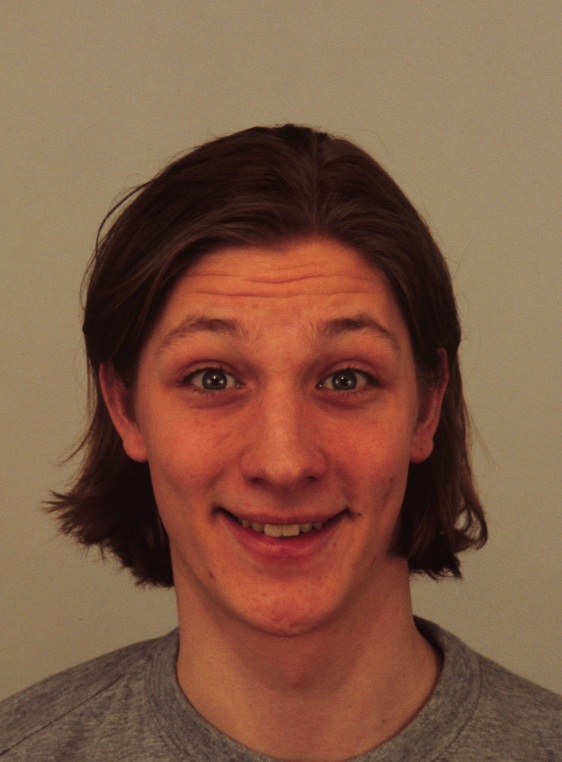
\includegraphics[scale=0.2]{exercise_3/paper/images/AM18HAS.JPG}
                    \caption{Face classified as happy by the Azure Emotion API}
                    \label{fig:happy_face}
            \end{figure}
        
        In the Microsoft Azure Emotion API there is a free pricing option which allows us to submit up to 20 images per minute as well as a standard plan with up to 10 calls per second. As Microsoft has a promotion for students, which gives 100€ free credit, we chose the premium plan. %which allows us to submit up to 10 images per second.
        
        We decided to steal the model behind this API because this is also considered in the paper by Correia-Silva et al.~\cite{copycat}. Hence, we are able to assess whether the performance of our extracted classifier is similar to the performance of the extracted classifier in the paper.
        
       As mentioned in the beginning of Section~\ref{sec:copycat} Azure could not recognise all of the faces in our data set and hence could not classify for each face an emotion. Therefore, we added to the 8 emotions a further class called 'no\textunderscore face'. Figure~\ref{subfig:emotions_original-labels} shows the proportion of the different classes in our data set. In Figure~\ref{subfig:emotions_azure-labels} the distribution after classification by Azure. As one can see Azure could not detect about $13\%$ of the human faces. We only performed a copycat attack with a problem domain dataset for this reason, since the Azure Emotion API in the current version does not allow us to extract emotions for images without an detected face.
       
       \begin{figure}[h!]
            \centering
            \begin{subfigure}[c]{0.45\textwidth}
                \centering
                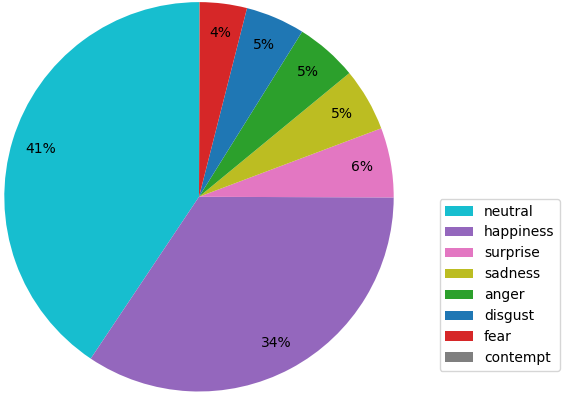
\includegraphics[width=0.95\textwidth]{exercise_3/paper/images/emotions_original-labels.png}
                \caption{Class Distribution}
                \label{subfig:emotions_original-labels}
            \end{subfigure}
            \begin{subfigure}[c]{0.45\textwidth}
                \centering
                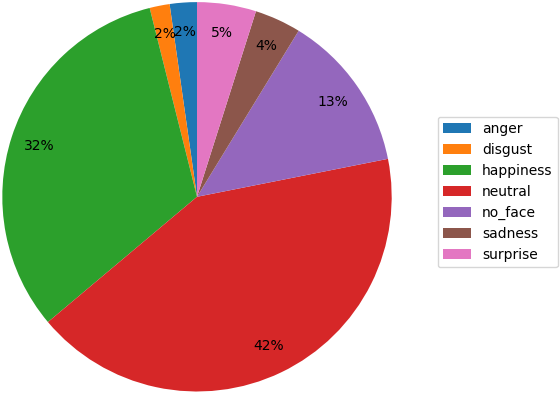
\includegraphics[width=0.95\textwidth]{exercise_3/paper/images/emotions_azure-labels.png}
                \caption{Classification of Azure}
                \label{subfig:emotions_azure-labels}
            \end{subfigure}
            \caption{Performance of Copycat Attack on first data set}
            \label{fig:emotions_distribution-labels}
        \end{figure}
        

    \subsection{Evaluation of the extracted Emotion Detection model}
        Since we had labeled data, we were able to compute the accuracy of the Microsoft Azure Emotion API. On the whole data set we obtained an accuracy of $0.76$.
        
        For testing the efficiency of our extracted model, we initially did a $75\%/25\%$ training/test split on our data set consisting of KDEF, AKDEF (see Subsection~\ref{subsec:dataset_KDEF-AKDEF}) and the one from Kaggle (see Subsection~\ref{subsec:dataset_kaggle-emotions}). As we had labeled data, we had to delete the labels before querying the Azure API as a black-box. From now on we will refer to the split for training the extracted model as attack set, since this set will be used to attack the target network.
        
        To learn the effect of the number if images in the training set, we used an incremental approach. We trained the model on progressively larger subsets of the training set, which were included in each other. Starting with a random sample $s_0$ of $2\,000$ images, the next training set $s_n$ consisted of $s_{n-1}$ and additional $1\,000$ randomly selected images, which are not already contained in $s_{n-1}$.
        
        In order to compare the performance of our extracted models to the target network we considered two measures:
        \begin{itemize}
            \item Accuracy: correctly classified faces with respect to the original labels.
            \item Equality: correctly classified faces with respect to the target network.  
        \end{itemize}
        %The CNN-classifier was trained by a Multi-layer Perceptron. As the copying algorithm used for this classifier was rather basic we mapped the size of the training set to the size of the subset of AKDEF/KDEF used to train our copy-cat.
        
        %In order to compare the performance of our copied classifier to the original we split the data set into a test and training set and looked at the accuracy resp. equality of our copied model, dependant on the size of the set used to train the model. We trained the model on progressively larger subsets of the training set, which were included in each other. 
        
        Figure~\ref{fig:performance-azure} shows the results of our tests. Overall it can be seen that the accuracy as well as the equality improve for larger training sets. The best value for the accuracy in our tests was $0.578$ which seems much better compared to the results from the paper with about $0.35$ depending on the attack data set. Nevertheless, the Azure Model used in the paper (which was an older version) also had an accuracy of around $0.351$. We also computed the accuracy of the Azure Emotion API on the test set and obtained an accuracy of $0.764$, which is much better than the accuracy recorded in the paper. Therefore our performance was $0.756$ compared to the target network.
        
        The extracted model using the whole attack set was was able to coincide on $70\%$ with the azure classifications on our test set. 
        
        \begin{figure}[h!]
            \centering
            \begin{subfigure}[c]{0.49\textwidth}
                \centering
                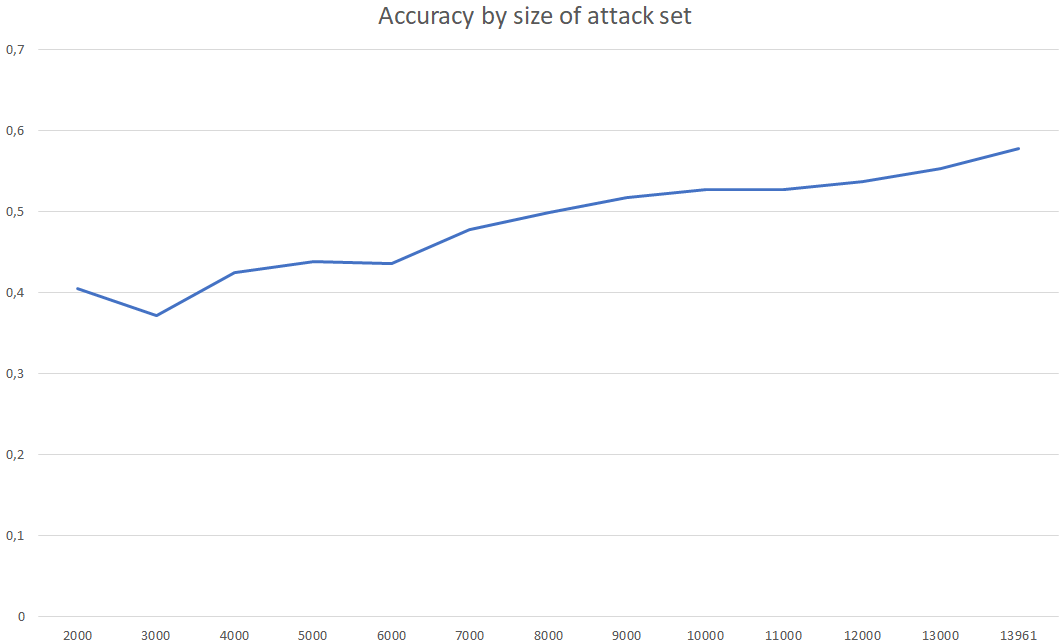
\includegraphics[width=1\textwidth]{exercise_3/paper/images/accuracy_copy_Azure.png}
                \caption{Accuracy of the extracted models}
                \label{fig:Accuracy_Azure}
            \end{subfigure}
            \begin{subfigure}[c]{0.49\textwidth}
                \centering
                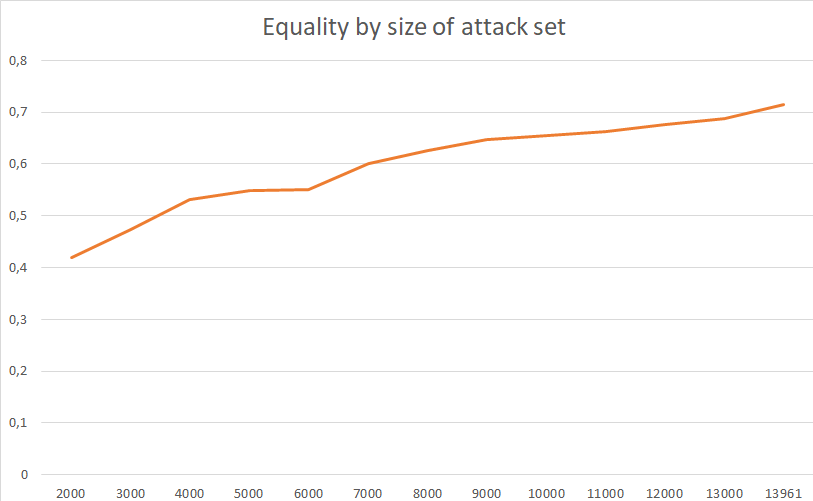
\includegraphics[width=1\textwidth]{exercise_3/paper/images/equality_copy_Azure.png}
                \caption{Equality of the extracted models}
                \label{fig:Equality_Azure}
            \end{subfigure}
            \caption{Performance of Copycat Attack on first data set}
            \label{fig:performance-azure}
        \end{figure}
        
        We took the offer for students and got $100$\$ of credit for free, which we used for the standard option. Therefore, we could label up to $10$ images per second but had to pay $1$\$ per $1\,000$ calls.
        
        Extracting a model using the whole data set took roughly one hour. About a third of this time was needed for training the model. The remaining time was for querying our target network for the labeling of our data set. 
        
        Using the free tier in Azure we would have needed about $16$ hours of time which is compared to the standard tier much longer, but still a reasonable timeframe. 

    \subsection{Data Sets: Cats vs. Dogs}
        In the following we have a binary classification problem, where we want to predict if a certain image contains a cat or a dog. 
        
        For building a model we will again combine several data sets. First of all, we need a training set for training the target network. Additionally, we will need images for the attack resp. test set. 
        
        \subsubsection{Dogs vs. Cats}\label{subsec:dataset_cats-dogs}
            Instead of using an already existing API, in this experiment we chose to train our own CNN to steal to make matters more interesting. We obtained the training set for building our target model from the Kaggle competition 'Dogs vs. Cats'~\cite{dogs-cats}. It contains in total $25\,000$ images including its labels, where half of the images picture cats and the other half dogs.
            
            Additionally, this Kaggle competition provided another data set with $12\,500$ pictures of cats and dogs, but without labels, as the goal of the competition was to predict these labels. Since the attack set does not need any labeled data, we decided to use this set as part of the attack set.
            
        \subsubsection{Cats} \label{subsec:dataset_cats}
            This data set is also from Kaggle~\cite{cats}. It contains roughly $10\,000$ images solely of cats in various positions. 
            In an additional file more information, like pointers to the eyes, ears and nose of the cats in the pictures, can be found. However we did not use them in any capacity. 
            
            We used this data set as part of the attack and test set. 
            
        \subsubsection{Stanford dogs data set} \label{subsec:dataset_dogs}
            The Stanford dogs data set ~\cite{dogs} was built using images from ImageNet in order to help categorize images. It contains $20\,580$ pictures purely of dogs. Additionally, it contains also classification for different breeds of dogs, but once again we did not use this information in out attack. 
            
            In our experiment this data set was used in the attack and test set.
            
        \subsubsection{Common objects in context data set}\label{subsec:dataset-coco}
            Since we construct the target network in this experiment by ourselves, we can use the copycat attack to it's full power and include non-problem domain data in our attack set. 
            For this we chose the Microsoft COCO (Common Objects in Context) data set~\cite{coco}, which is known for object detection, segmentation and captioning. With a size of about $118\,000$ images it is a large data set. 
            
            These images will only be used in the attack set, since the classification problem is to decide if a picture shows a dog or a cat, but not to decide if it is something else. Moreover, since the images in this data set do not contain to our problem domain and compared to the number of our problem-domain data is much bigger, we decided not to use the whole data set. 
    
    \subsection{Target Network}
        The targeted CNN was trained using the Dogs vs. Cats data set from Kaggle (see Subsection~\ref{subsec:dataset_cats-dogs}). We build a CNN consisting of 3 Convolutional layer blocks and a fully connected layer. In each Convolutional layer block we are applying
        \begin{itemize}
            \item 2D convolutions two times with a kernel size of 3 and padding value of 1,
            \item Batch Normalisation,
            \item ReLU as activation function,
            \item Max Pooling with a kernel size of 2 and a stride of 2. 
        \end{itemize}
        In the fully connected layer we are applying the following methods several times:
        \begin{itemize}
            \item Dropout with $p=0.1$ (probability of an element to be zeroed),
            \item linear transformation,
            \item ReLU.
        \end{itemize}
       
       We trained the target model for 10 epochs and using Stochastic Gradient Descent with a Step Down policy for the learning rate and CrossEntropyLoss as criterion. In the augmentation step we resized the images. 
       
       This model achieved an accuracy of $0,821$ on the test data set (see Subsection~\ref{subsec:evaluation-cats-dogs} for more detailed description and analysis). 
       
    \subsection{Evaluation of the extracted Cats vs. Dogs model}~\label{subsec:evaluation-cats-dogs}
        As our test set we made a $25\%$ split on the Cats (see Subsection~\ref{subsec:dataset_cats}) and the Dogs (see Subsection~\ref{subsec:dataset_dogs}) data set. 
        
        We extracted the model in two different ways. First, we used only images that are part of the domain, therefore pictures of cats and dogs, in the attack set. For this we combined the remaining $75\%$ of the Cats and Dogs images with the unlabeled data of the Cats vs. Dogs data set (see Subsection~\ref{subsec:dataset_cats-dogs}). 
        For evaluation we proceeded similarly to the Emotion Detection problem. We started with a random subset with $3\,000$ images as our attack set and extracted a model. Then we iteratively increased the size of the attack size by $3\,000$ images and in each step extracted another model until we used all of the available images for the model-stealing attack.
        
        Moreover, we also experimented also with a mixture of non-problem domain (short NPD) images and problem domain (short PD) images in the attack set. For this we added half of the COCO data set (see Subsection~\ref{subsec:dataset-coco}) to our attack set. The ratio between the PD and NPD instances in the total set was $2:5$.
        The testing phase including NPD images was similar to the PD case. As we had much more images in this case, we started with an initial attack set of $5\,000$ images and increased its size in each step by $10\,000$ pictures.
        
        Our experiments had the following results. Figure~\ref{fig:accuracy_cat} shows the accuracy for each of the two approaches with increasing number of instances in the attack set. As we can see in the case, where only PD data is used to attack, there is a slight increase for larger attack sets from $0.632$ to $0.768$, but the difference is not very much. 
        
        Considering the second case in Figure~\ref{fig:accuracy_cat_PD+NPD}, where also NPD data is included, we can see that this looks similar to the other approach. The accuracy increases from $0.673$ to $0.791$.
        
        The accuracy of the target model on the same test set was $0,821$. 
        Comparing the accuracy of the extracted models in our tests to the accuracy of the target CNN we can see that this measure is very close to the original one.
        
        \begin{figure}[h!]
            \centering
            \begin{subfigure}[c]{0.49\textwidth}
                \centering                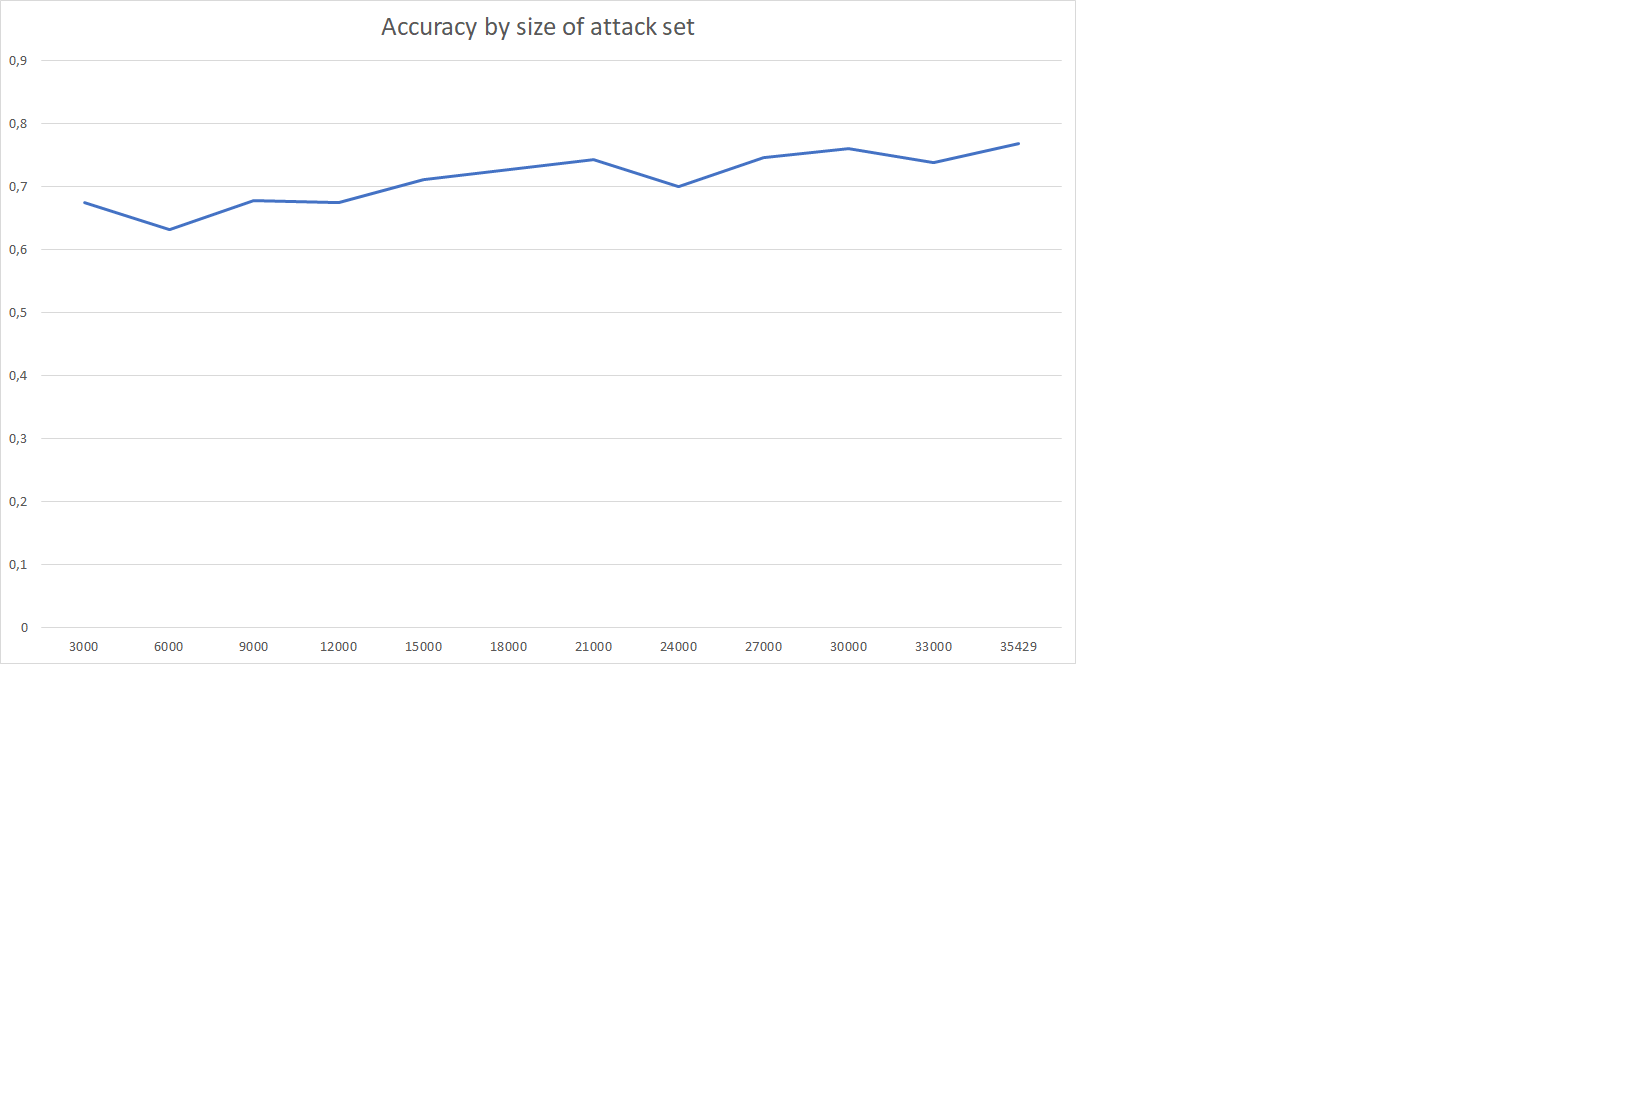
\includegraphics[width=1\textwidth]{exercise_3/paper/images/Accuracy_copy_cat_domain.png}
                \caption{Accuracy using only PD data}
                \label{fig:accuracy_cat_PD}
            \end{subfigure}
            \begin{subfigure}[c]{0.49\textwidth}
                \centering                \includegraphics[width=1\textwidth]{exercise_3/paper/images/Accuracy_copy_cat.png}
                \caption{Accuracy including also NPD data}
                \label{fig:accuracy_cat_PD+NPD}
            \end{subfigure}
            \caption{Accuracy of Copycat Attack on second data set}
            \label{fig:accuracy_cat}
        \end{figure}

        Furthermore, we will consider the equality of our extracted model. In Figure~\ref{fig:equality_cat} we can see that the two graphs for both approaches look very similar. For a larger attack set the equality can be improved up to $0.864$. This means, compared to the previous Emotion Detection problem, we were able to copy the model in this setting better in these tests and on the given data.
        
         \begin{figure}[h!]
            \centering
            \begin{subfigure}[c]{0.49\textwidth}
                \centering                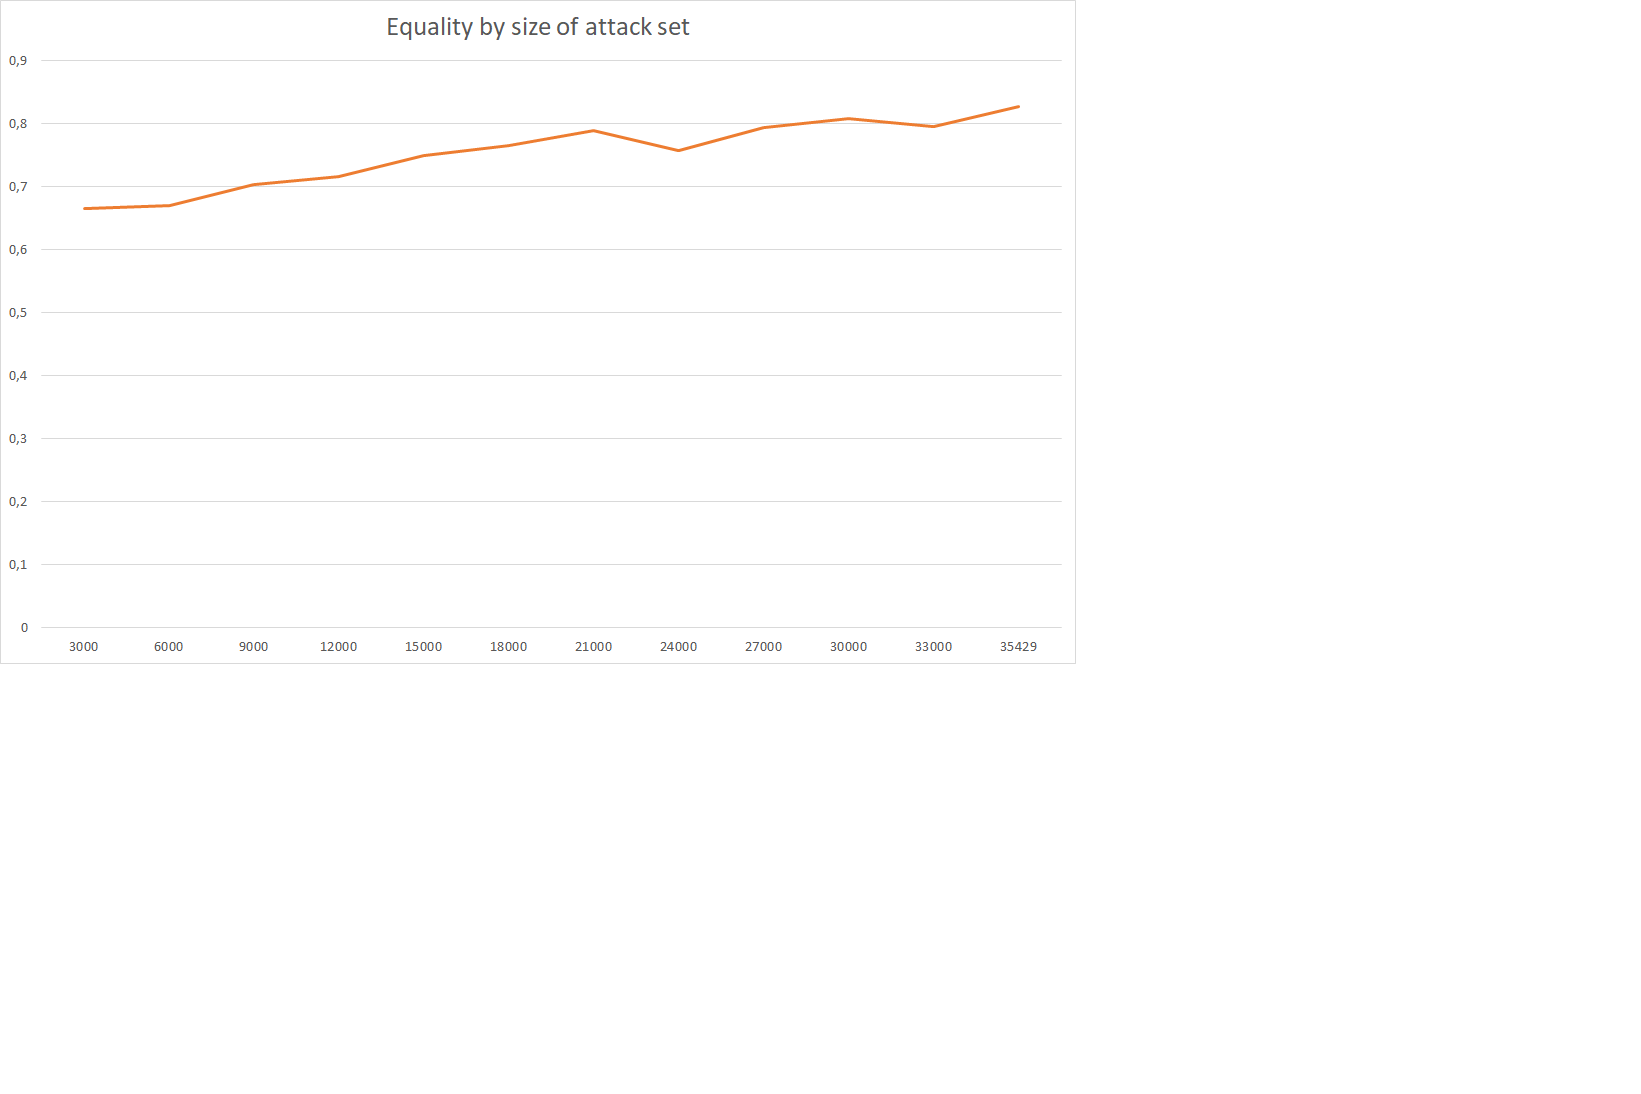
\includegraphics[width=1\textwidth]{exercise_3/paper/images/Equality_copy_cat_domain.png}
                \caption{Equality using only PD data}
                \label{fig:Equality_cat_PD}
            \end{subfigure}
            \begin{subfigure}[c]{0.49\textwidth}
                \centering                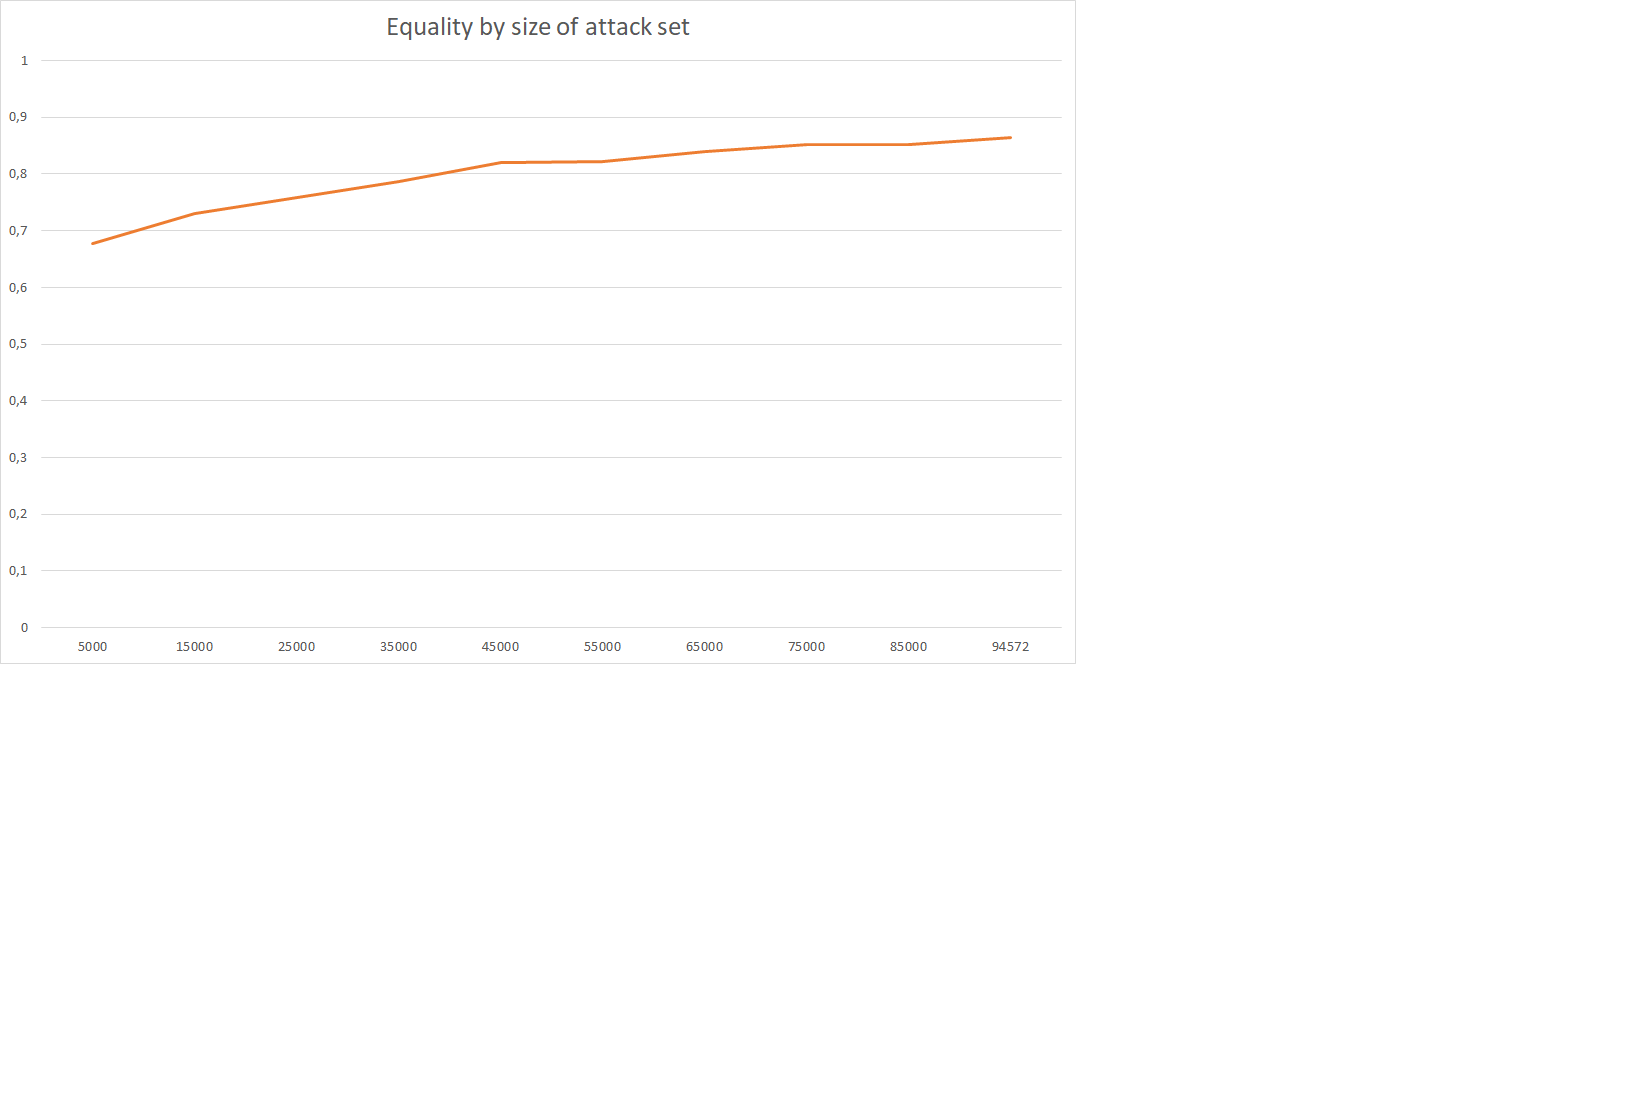
\includegraphics[width=1\textwidth]{exercise_3/paper/images/Equality_copy_cat.png}
                \caption{Equality including also NPD data}
                \label{fig:equality_cat_PD+NPD}
            \end{subfigure}
            \caption{Equality of Copycat Attack on second data set}
            \label{fig:equality_cat}
        \end{figure}
        
        In addition to that, we will also look at how much time it takes to train the extracted model for an attack set of certain size. As it can be seen in Figure~\ref{fig:time_cat} the time for training the models grew roughly linear with the size of the attack set in our tests. The largest attack set containing $94\,572$ images needed about $24$ minutes to perform the attack, i.e. to build the extracted model.
        
        \begin{figure}[h!]
            \centering      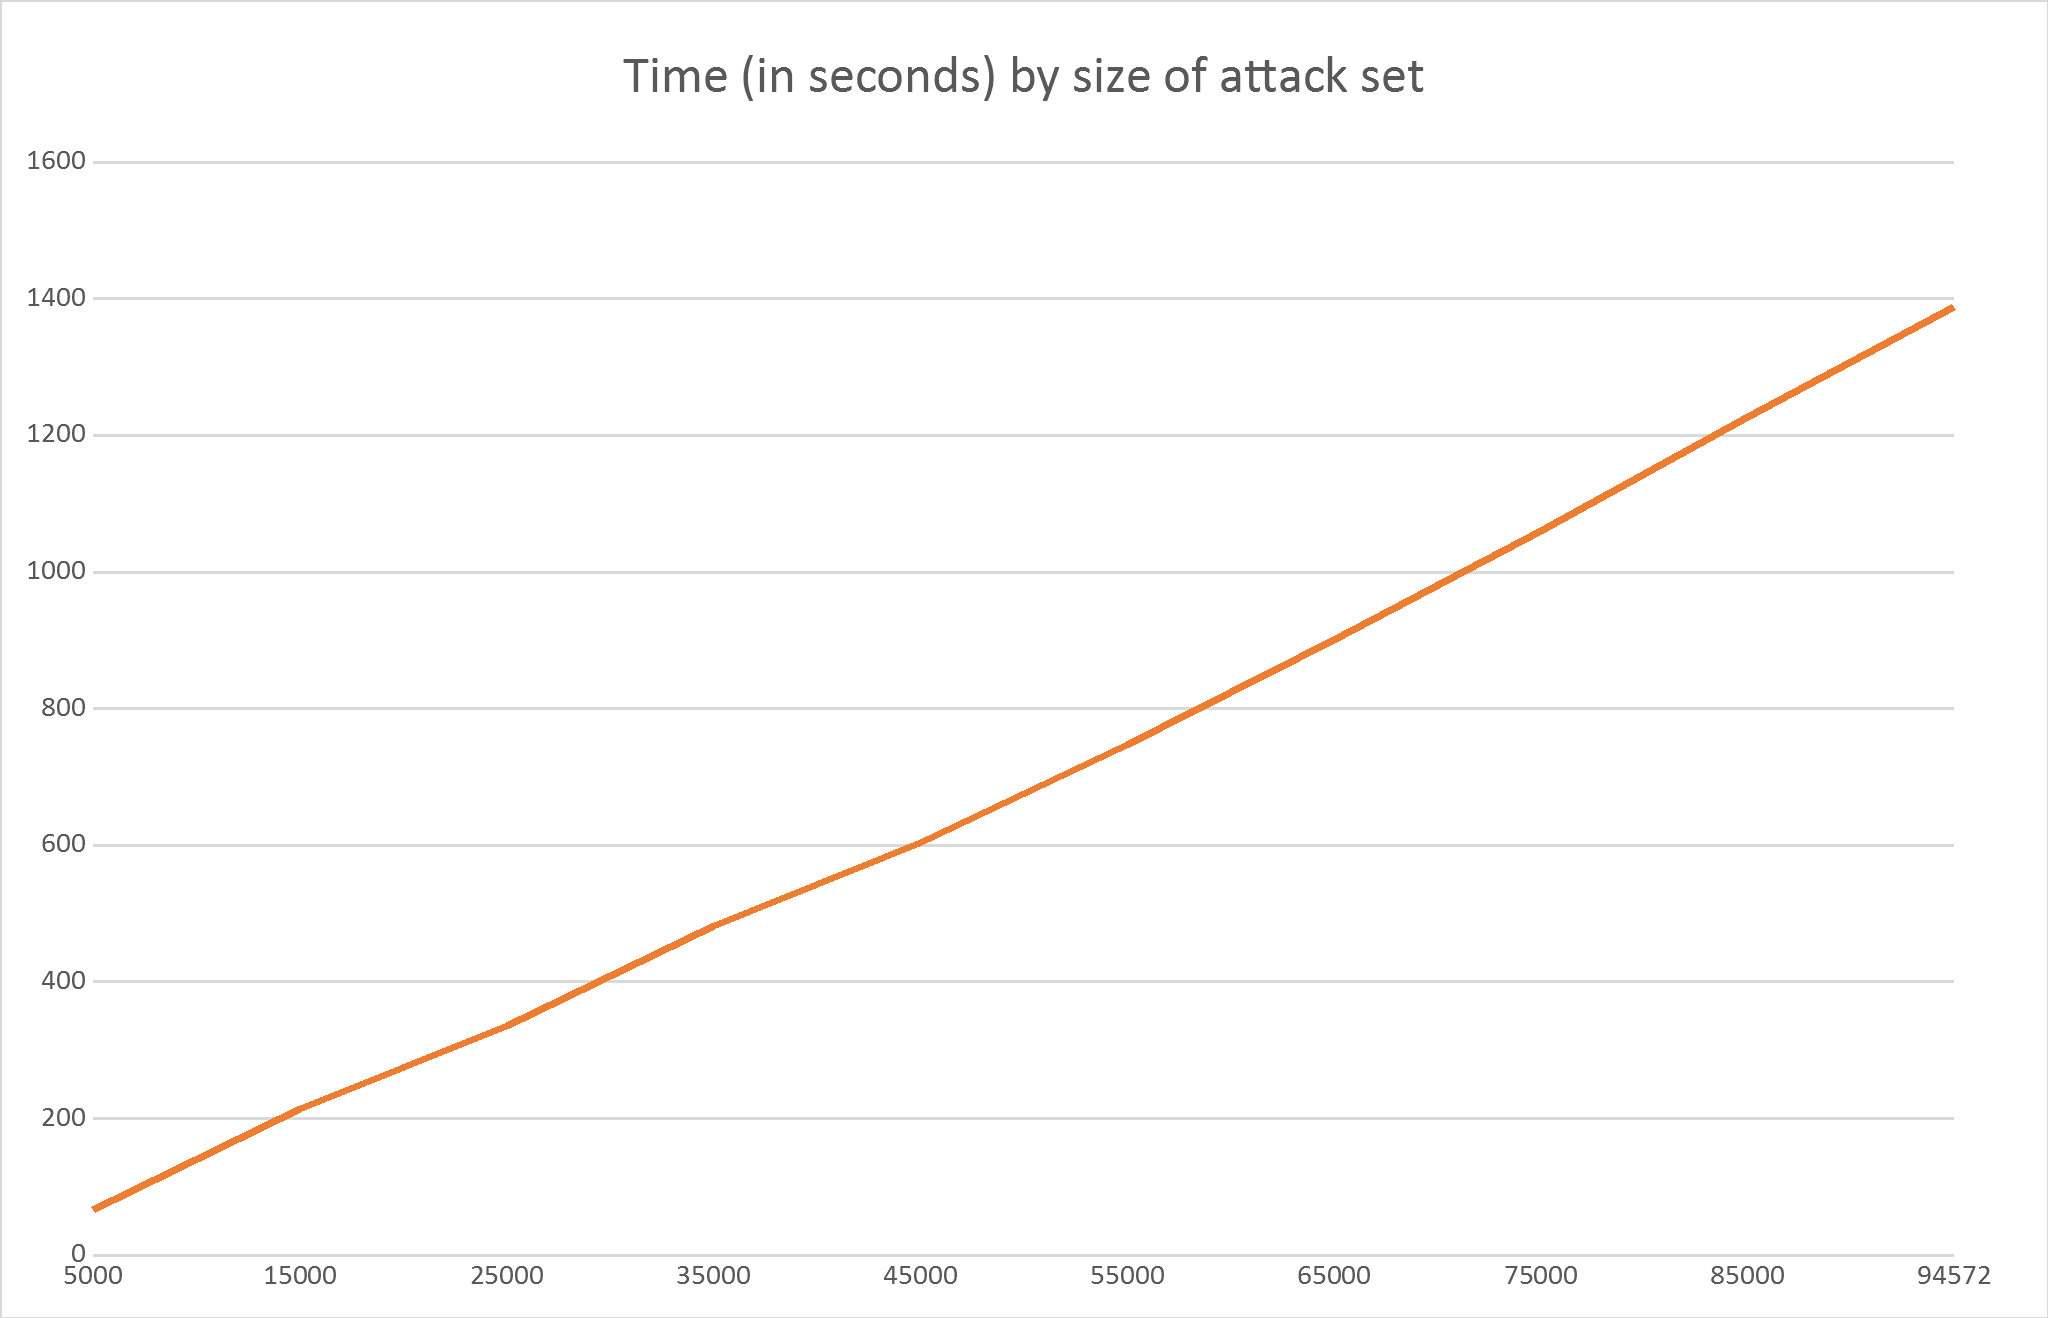
\includegraphics[width=0.65\textwidth]{exercise_3/paper/images/Time_copy_cat.png}
            \caption{Time needed to extract a model}
            \label{fig:time_cat}
        \end{figure}
        
        Summarizing it can be said that for a fixed number of PD data, adding NPD images improves the accuracy and equality of the extracted model. But since more queries to the target network are required when adding NPD data, the time needed for building the model increases. Hence, there is a trade-off between the performance of the model and the costs.
        
            
\section{Decision Tree Path-Finding Attack}
    As the name suggests this model stealing attack targets decision tree models. Such a model divides the input space into several discrete partitions. The idea behind the decision tree path-finding attack is to vary the values of each feature bit by bit and then to query the black-box to find the values at which the tree splits. In Algorithm~\ref{alg:DT-attack} you can find a rough sketch of this attack. In this pseudocode let $Q$ be the set of unprocessed queries and $P$ the set of explored leaves with their classification value.
    
    \begin{algorithm}
        \caption{Path-finding attack for decision trees}
	    \begin{algorithmic}[1]
%		    \State Let $Q$ be the set of unprocessed queries;
%		    \State Let $P$ be the set of explored leaves with their classification;
		    \State Add a random first query to $x_{init}$ to $Q$;
		    \State While $Q\neq\emptyset$ process $x\in Q$;
		    \State Do binary search over the continous features and check whether a new leaf can be discovered;
		    \State in this way explore the continuous features and variate the discrete features to find all leaves;
	    \end{algorithmic}
	    \label{alg:DT-attack}
    \end{algorithm}
    
    A weakness of this approach is that for two instances which e.g. only differ in a single feature, the target decision tree leads to different leaves which are classified as the same, the difference may not be registered in the extracted model.
    
    We carried out our experiments using GCP e2-highmem-16 offered by the Google Cloud Platform running on Ubuntu 20.04.
    
    \subsection{Models}
        Since this model stealing attack does not use attack sets to get the model (like the previous one) to confess its knowledge, we looked at publicly available decision tree models from BigML instead of data sets.
        
        Moreover, we decided to consider the models from the paper to find out if this model stealing attack implemented exactly as in the paper but performed in a different setting yields to exactly the same extracted model or if it leads to any differences.
        
        \subsubsection{US IRS 2008 tax data patterns}
            The decision tree for US IRS 2008 tax data patterns~\cite{tax} was generated using data from tax returns filed in the US in 2008. The decision tree aims to predict the home state of the tax payer depending, e.g. on the unemployment compensation, real estate taxes or the tax due at time of filing. 
        
        \subsubsection{Steak survey}
            
            This model was based on data from a \hyperlink{https://fivethirtyeight.com/features/how-americans-like-their-steak/}{FiveThirtyEighty survey}, which asked a lot of general questions as well as how they liked their steak prepared (Rare, Medium-rare, Medium, Medium-well, Well). 
            
        \subsubsection{Bitcoin price} 
            https://bigml.com/user/czuriaga/gallery/model/51ccb90a035d07603900039e
            Was macht der TREEEE?????
        
        \subsubsection{Email Importance}
            https://bigml.com/user/louisdorard/gallery/model/52fa8aa60c0b5e6d4a0030c1
        
            This model was built using Email data collected from the users own inbox. The importance was set by Gmail. Using a variety of features including length of the mail and whether the mail was sent by a contact, the tree classifies the importance.
            
        \subsubsection{gss survey}
            Find das model ned
            
        \subsubsection{med price}
            Find ich ned
            
    \subsection{Evaluation}
        ...

\section{Conclusions}
    The copy-cat method in general performed extremely well, getting an equality of roughly $0,7$ even on the rather complex Microsoft Azure emotional API in less than one hour and using a rather small attack set. While using only instances that are part of the problem domain worked better on similar attack set sizes, finding instances that are not part of the problem domain is an easier task in general and still works pretty well. Taking this into consideration, in case that the number of queries on can make to the blackbox is severely limited or run time is an important factor, one should rely mainly on problem domain instances. Should this not be the case non-problem domain instances allow for a quick assembly of a large data set that can extract a model reasonably well.

\printbibliography

\end{document}